%%%%%%%%%%%%%%%%%%%%%%%%%%%%%%%%%%%%%%%%%
% baposter Portrait Poster
% LaTeX Template
% Version 1.0 (15/5/13)
% Created by: % Brian Amberg (baposter@brian-amberg.de)
% License: % CC BY-NC-SA 3.0 (http://creativecommons.org/licenses/by-nc-sa/3.0/)
%%%%%%%%%%%%%%%%%%%%%%%%%%%%%%%%%%%%%%%%%

%----------------------------------------------------------------------------------------
%	PACKAGES AND OTHER DOCUMENT CONFIGURATIONS
%----------------------------------------------------------------------------------------

\documentclass[a0paper,portrait]{baposter}
%a0 paper = 84.1 x 118.9 cm

\usepackage[font=small,labelfont=bf]{caption} % Required for specifying captions to tables and figures
\usepackage{booktabs} % Horizontal rules in tables
\usepackage{relsize} % Used for making text smaller in some places
\usepackage{textcomp}   % to use+- symbol in text
\usepackage[none]{hyphenat} % avoid cut words (hyphenation)

\graphicspath{{figures/}} % Directory in which figures are stored

\definecolor{bordercol}{RGB}{40,200,40} % Border color of content boxes
\definecolor{headercol1}{RGB}{110, 200, 50} % Background color for the header in the content boxes (left side)
\definecolor{headercol2}{RGB}{34, 120, 15} % Background color for the header in the content boxes (right side)
\definecolor{headerfontcol}{RGB}{0,0,0} % Text color for the header text in the content boxes
%\definecolor{boxcolor}{RGB}{100,200,50} % Background color for the content in the content boxes
\definecolor{boxcolor}{rgb}{0.82, 0.94, 0.75}

\newcommand{\up}[1]{\textsuperscript{#1}}     %for have up{} for authors
    


\begin{document}


\background{ % Set the background to an image (background.pdf)
\headerheight=2cm  %with large title
%\headerheight=2.5cm  %Height of the main poster header as a length
\begin{tikzpicture}[remember picture,overlay]
\draw (current page.north west)+(-3em,1em) node[anchor=north west]
{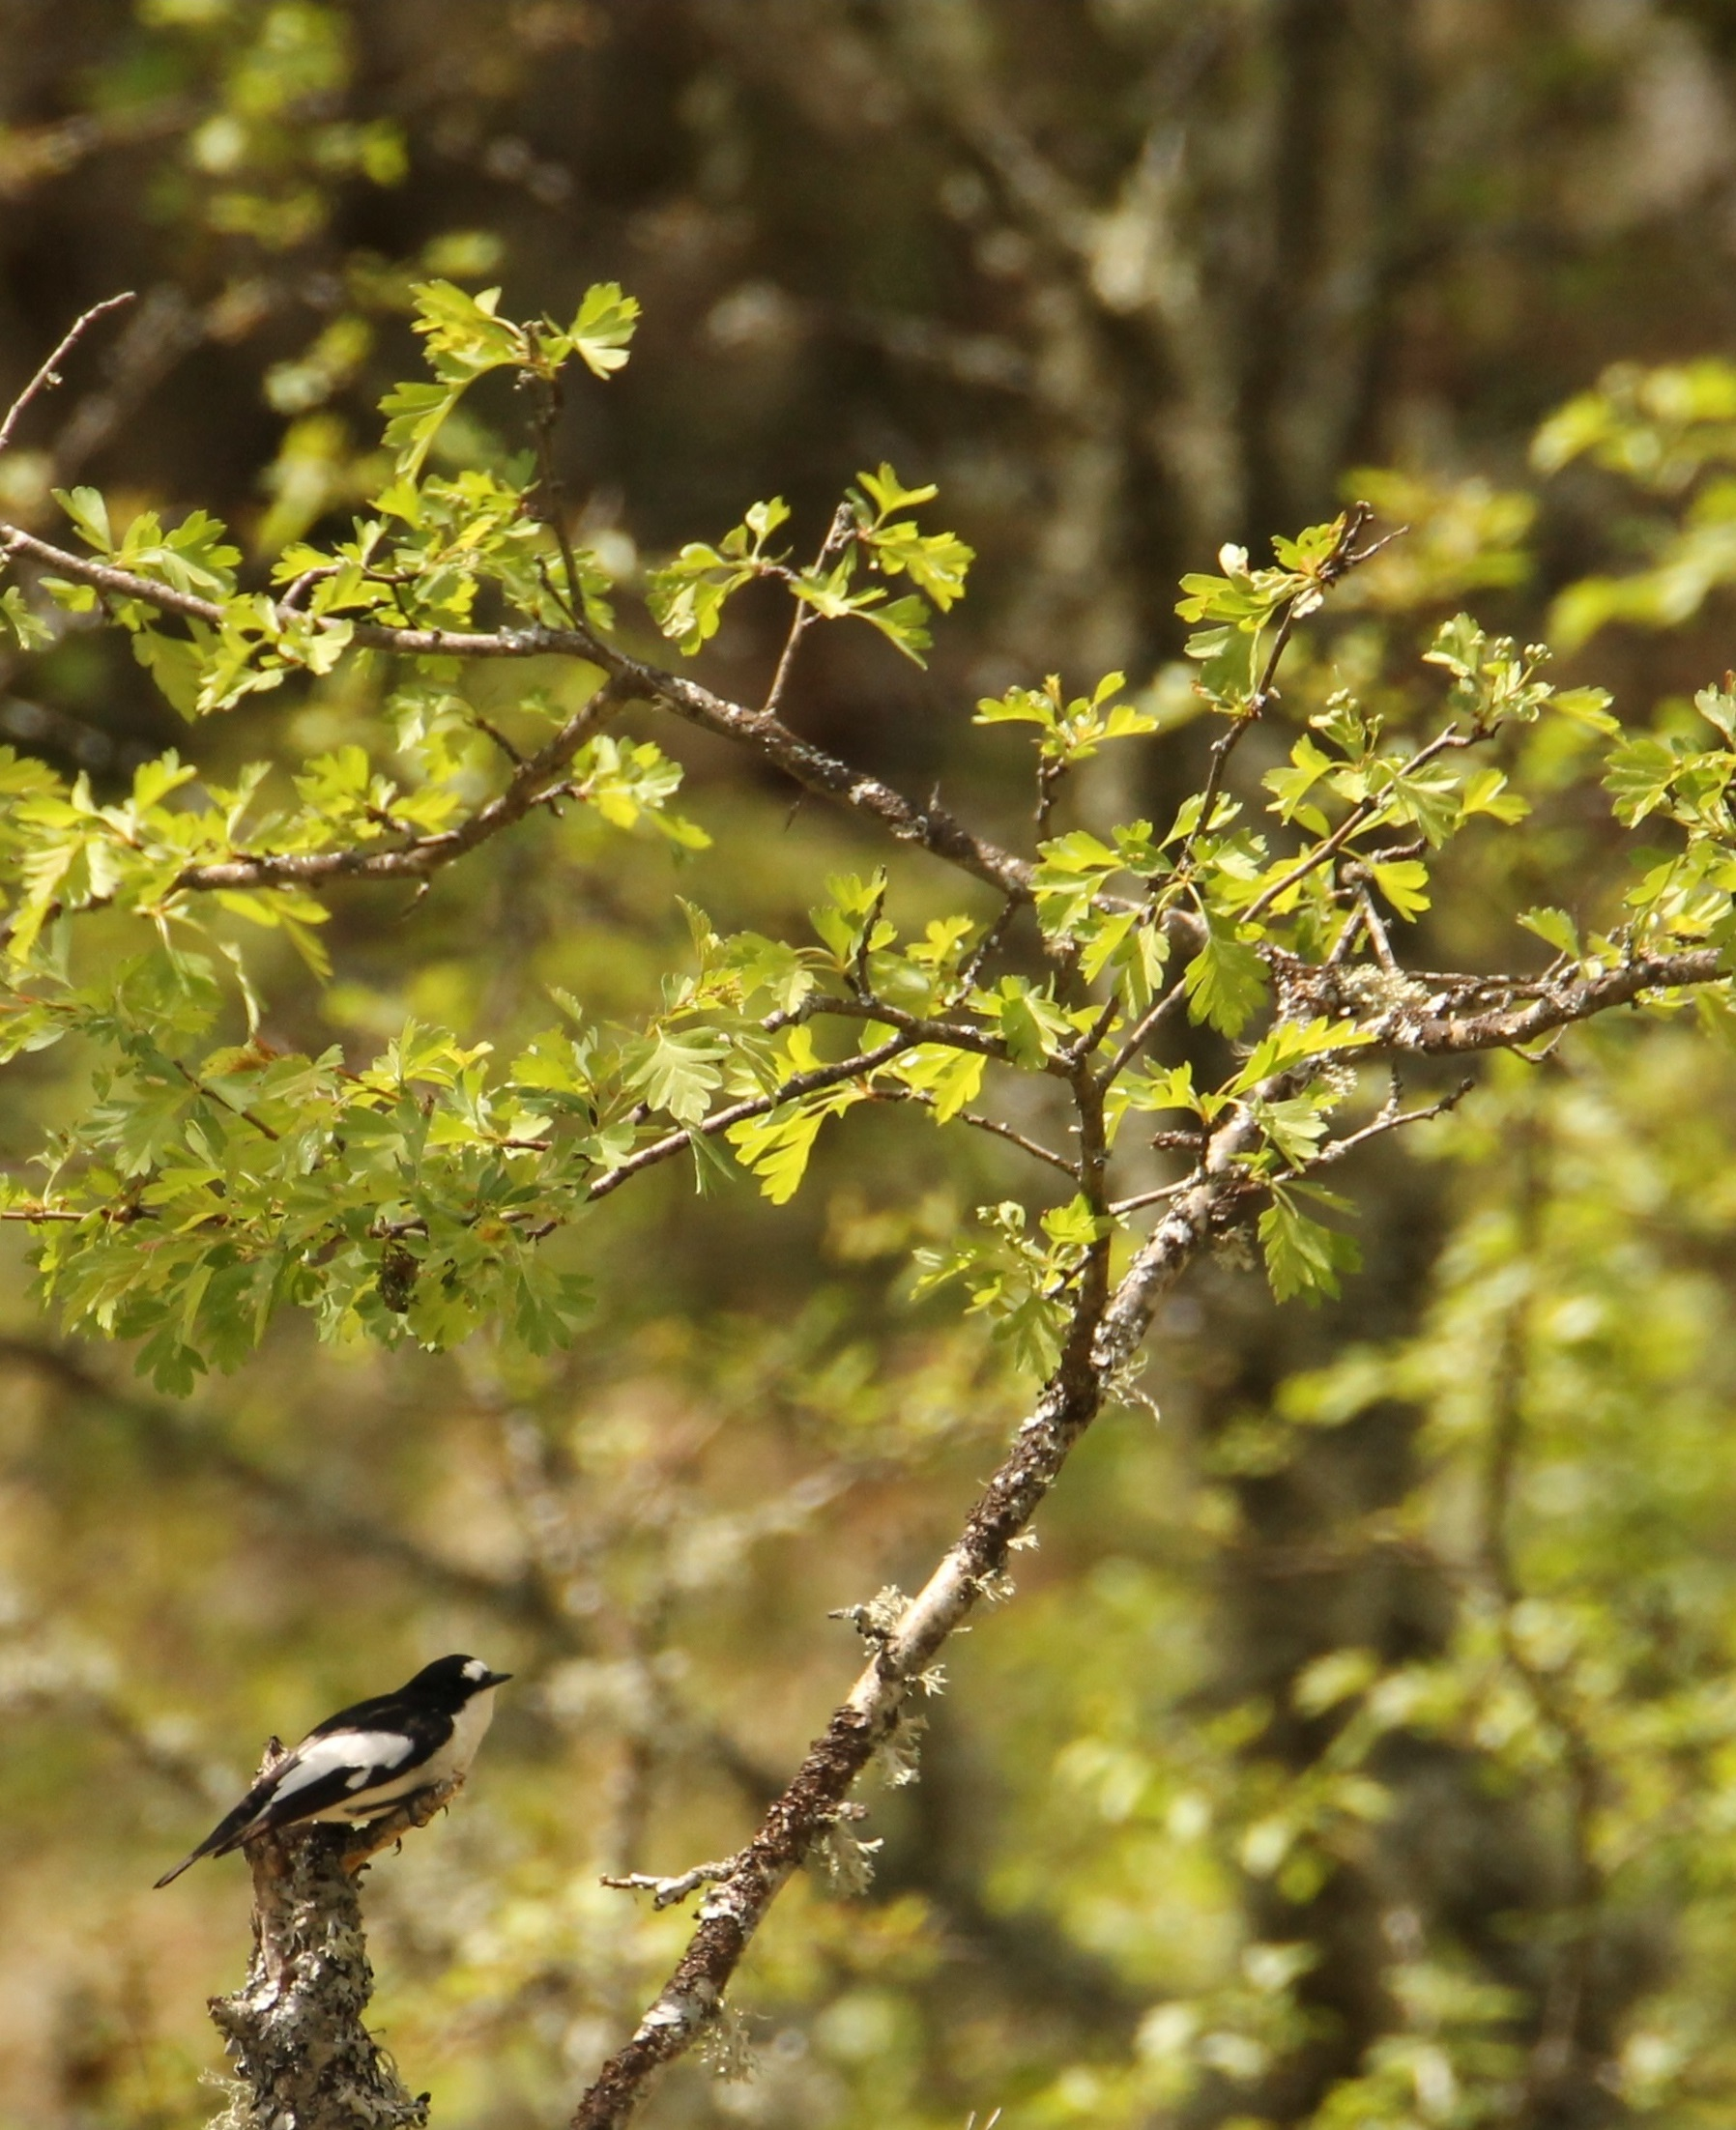
\includegraphics[height=1.05\textheight]{background}};%the header for the poster title and authors
%\fill [fill=white] (current page.north west) rectangle ([yshift=-\headerheight] current page.north east);% white rectangle title
\end{tikzpicture}
}

\begin{poster}{
grid=false,
borderColor=bordercol, % Border color of content boxes
headerColorOne=headercol1, % Background color for the header in the content boxes (left side)
headerColorTwo=headercol2, % Background color for the header in the content boxes (right side)
headerFontColor=headerfontcol, % Text color for the header text in the content boxes
boxColorOne=boxcolor, % Background color for the content in the content boxes
headershape=roundedright, % Specify the rounded corner in the content box headers
headerfont=\Large\sf\bf, % Font modifiers for the text in the content box headers
textborder=none,  %can be rectangle to have borderline
background=user,
headerborder=none, % Change to closed for a line under the content box headers
boxshade=plain
}
{}
%
%----------------------------------------------------------------------------------------
%	TITLE AND AUTHOR NAME
%----------------------------------------------------------------------------------------
%
%P-0265 poster number
{\sf\bf\color{white}The relative contribution of multiple agents of selection on laying date in a Mediterranean population of pied flycatchers}
% {\sf\bf\color{white} The contribution of climatic factors to the selection on laying date in\textit{Ficedula hypoleuca}} % Poster title
{\vspace{1em}\color{white} Justine Le Vaillant \up{1,2}, Jaime Potti\up{2}, Carlos Camacho \up{2}, Jes\'{u}s Mart\'{i}nez-Padilla\up{1} \\    % Author names 
{\smaller \up{1}UMIB - Research Unit of Biodiversity, University of Oviedo, Spain \\ \up{2}Department of Evolutionary Ecology, Estaci\'{o}n Biol\'{o}gica de Do\~{n}ana-CSIC, Sevilla, Spain }} % Author email addresses
{
\includegraphics[scale=0.07]{logo_labo}} % University/lab logo

%----------------------------------------------------------------------------------------
%	INTRODUCTION
%----------------------------------------------------------------------------------------

\headerbox{Introduction}{name=introduction,column=0,row=0.04}{
%\headerbox{Introduction}{name=introduction,column=0,row=0.02}{
Identifying environmental factors that drive selection in natural populations will help to unravel and anticipate evolutionary changes in wild animal populations facing global change.\\
The timing of reproduction (laying date) in birds is widely used to compare evolutionary responses to environmental change.
}

%----------------------------------------------------------------------------------------
%	MATERIALS AND METHODS
%----------------------------------------------------------------------------------------

\headerbox{Materials and Methods}{name=methods,column=0,below=introduction}{
We explored the relative influence of 16 environmental variables on the form, strength and direction of selection on laying date, in a population of pied flycatchers \textit{Ficedula hypoleuca} breeding in central Spain between 1987 and 2016. \\
We quantified yearly selection gradients of laying date from the linear regression \cite{lande1983measurement} between laying date and fitness proxies (clutch size, number of fledglings and recruits, recruitment rate and female survival). Models with climatic factors are applied to these gradients and selected by the AIC criteria.
}

%----------------------------------------------------------------------------------------
%	CONCLUSION
%----------------------------------------------------------------------------------------

\headerbox{Conclusion}{name=conclusion,column=0,below=methods}{
Our population of pied flycatchers does not display a trend in laying date over time, being in disagreement with the advance in laying date reported in north European populations\cite{Both2001a}.  

We found that two abiotics factors - the North Atlantic Oscillation index in winter and the variation of temperature in April - influence the most the strength and direction of selection on laying date. 

The heterogeneity of climatic variation over time explains selection on laying date, but the lack of temporal trends on those climatic factors results in a smaller shift in laying date overtime compared to northern populations facing Global Change.
}

%----------------------------------------------------------------------------------------
%	REFERENCES
%----------------------------------------------------------------------------------------

\headerbox{References}{name=references,column=0,below=conclusion}{

\smaller % Reduce the font size in this block
\renewcommand{\section}[2]{\vskip 0.05em} % Get rid of the default "References" section title
%\nocite{*} % Insert publications even if they are not cited in the poster

\bibliographystyle{unsrt} %complete name authors

\bibliography{library} % Use the bibliography file - !Lande&Arnold 1983 + Both et al 2004
}

%----------------------------------------------------------------------------------------
%	ACKNOWLEDGEMENTS
%----------------------------------------------------------------------------------------

\headerbox{Acknowledgements}
%{name=acknowledgements,column=0,below=references}{
{name=acknowledgements,column=0,above=bottom}{ 
\smaller % Reduce the font size in this block
Project CGL2015-70639-P from Spanish Government.\\ 
Grant FPI-MICINN (BES-2016-077694) from Spanish Ministry of Economy and Competitiveness to JLV.
\begin{center}
{
\includegraphics[scale=0.3]{logo-ministerio-de-economia-industria-y-competitividad}} 
\end{center}
}

%----------------------------------------------------------------------------------------
%	RESULTS 1
%----------------------------------------------------------------------------------------

\headerbox{Results - Change in laying date} %{name=results1,span=2,column=1,row=0.02}{% To reduce this block to 1 column width, remove 'span=2'
{name=results1,span=2,column=1,row=0.04}{% To reduce this block to 1 column width, remove 'span=2'

Laying date does not display a significant advance over time (Figure 1, r=-0.08\textpm0.07, n=2935, P=0.22), just a shift in the mean laying date of around 3.7 days in three decades. 

%------------------------------------------------

\begin{center}
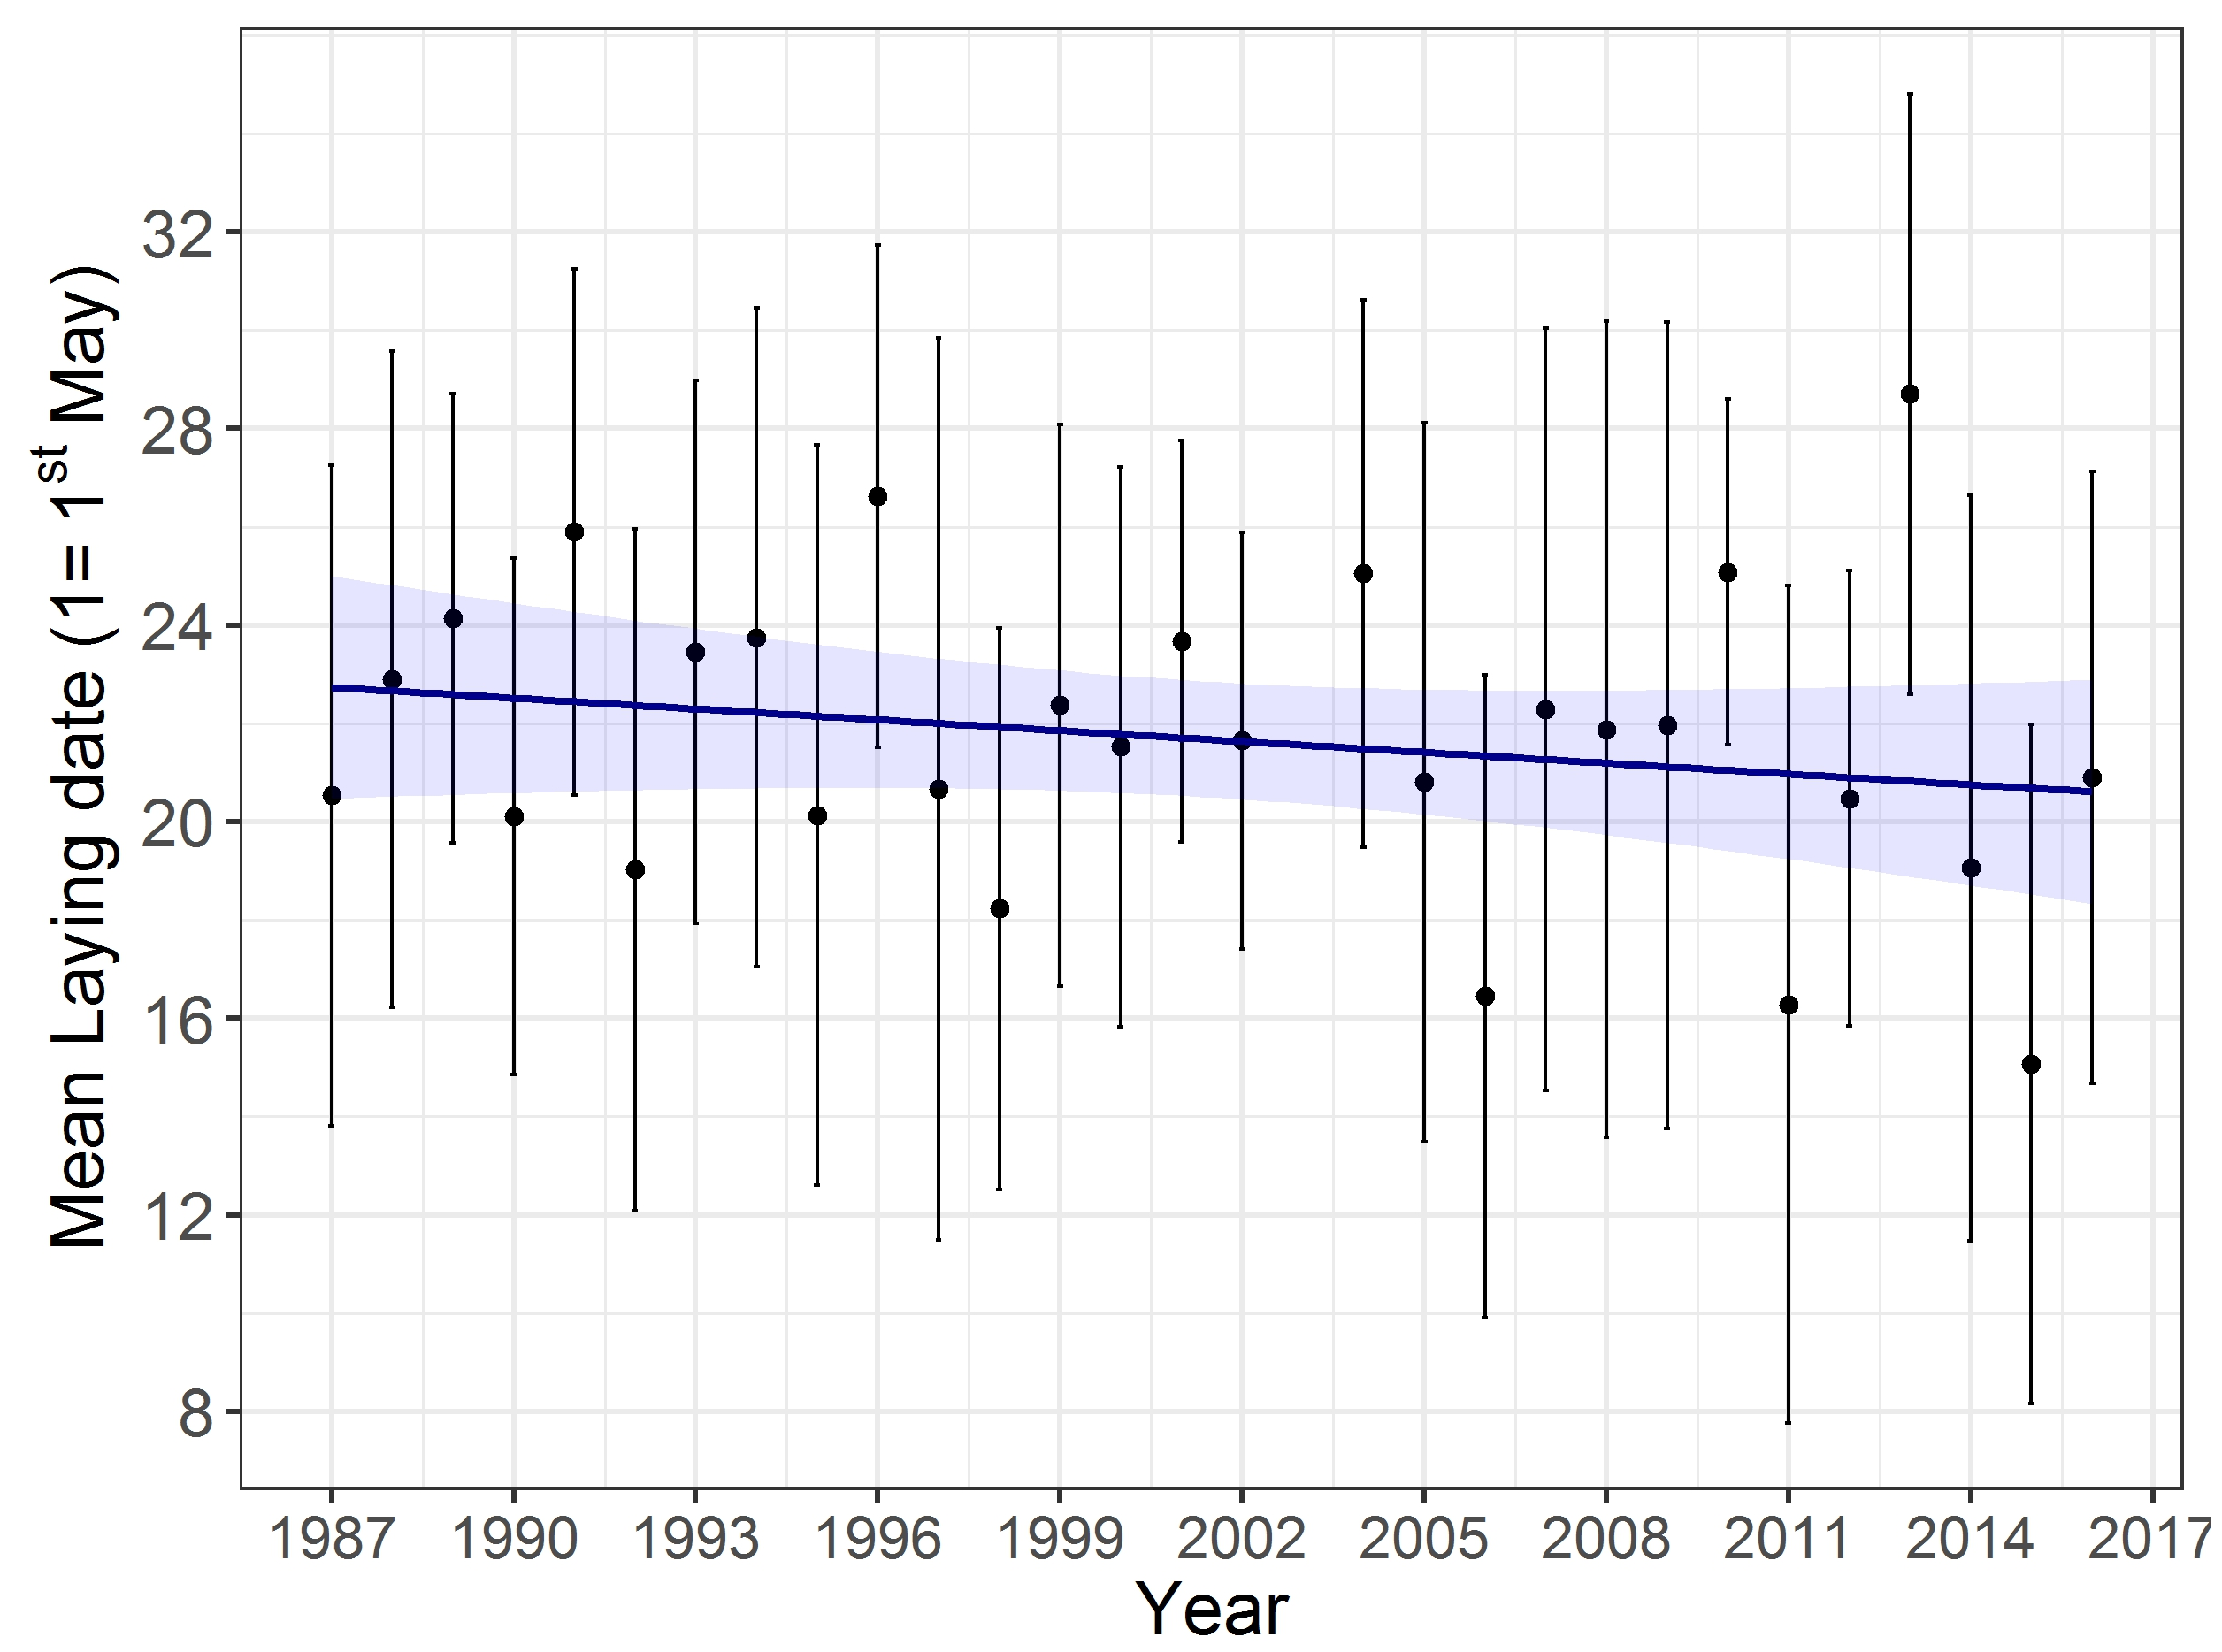
\includegraphics[width=0.47\linewidth]{Figure1_1}
%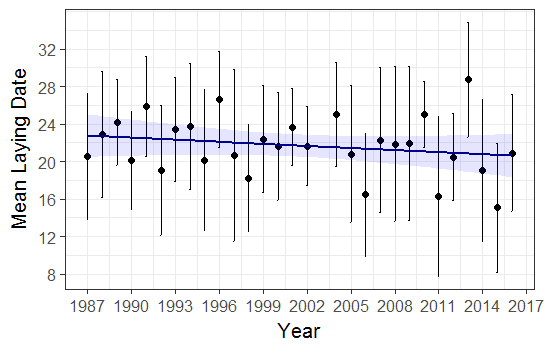
\includegraphics[width=0.5\linewidth]{Figure1}
\captionof{figure}{Change in laying date over time (annual laying date [1=1\textsuperscript{st} May] \textpm se).}
\end{center}

}
%----------------------------------------------------------------------------------------
%	RESULTS 2
%----------------------------------------------------------------------------------------

\headerbox{Results - Selection on laying date} {name=results2,span=2,column=1,below=results1, above=bottom}{% To reduce this block to 1 column width, remove 'span=2'

Estimates of directional selection gradients $\beta$ reveal that selection on laying date was negative for all reproductive fitness components assessed (Figure 2).
Early breeding birds were positively selected since they laid more eggs (P<0.01, df=2009), produced more fledglings (P<0.01, df=2089), more recruits (P=0.01, df=1698) and had a higher recruitment rate of their offspring (P=0.01, df=1697). Female survival was not associated with the date of laying (P=0.78, df=1945).
 

%------------------------------------------------

\begin{center}
%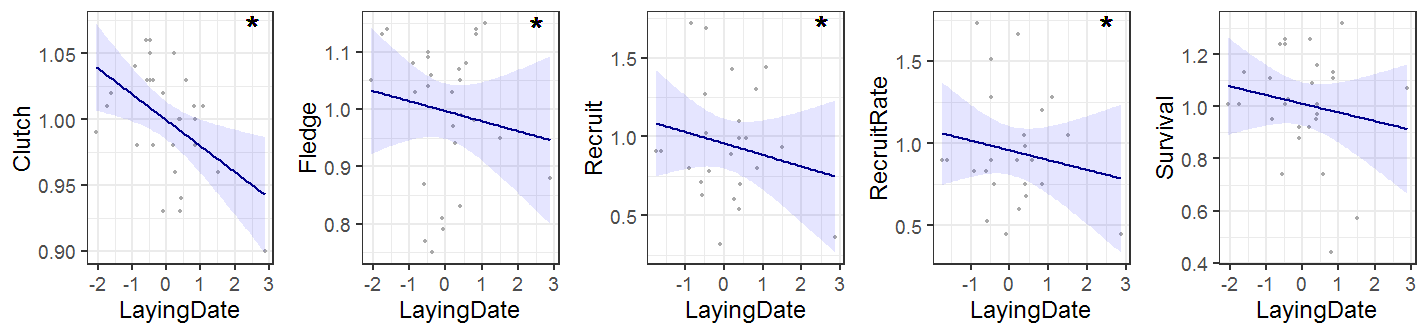
\includegraphics[width=0.90\linewidth]{Figure2}
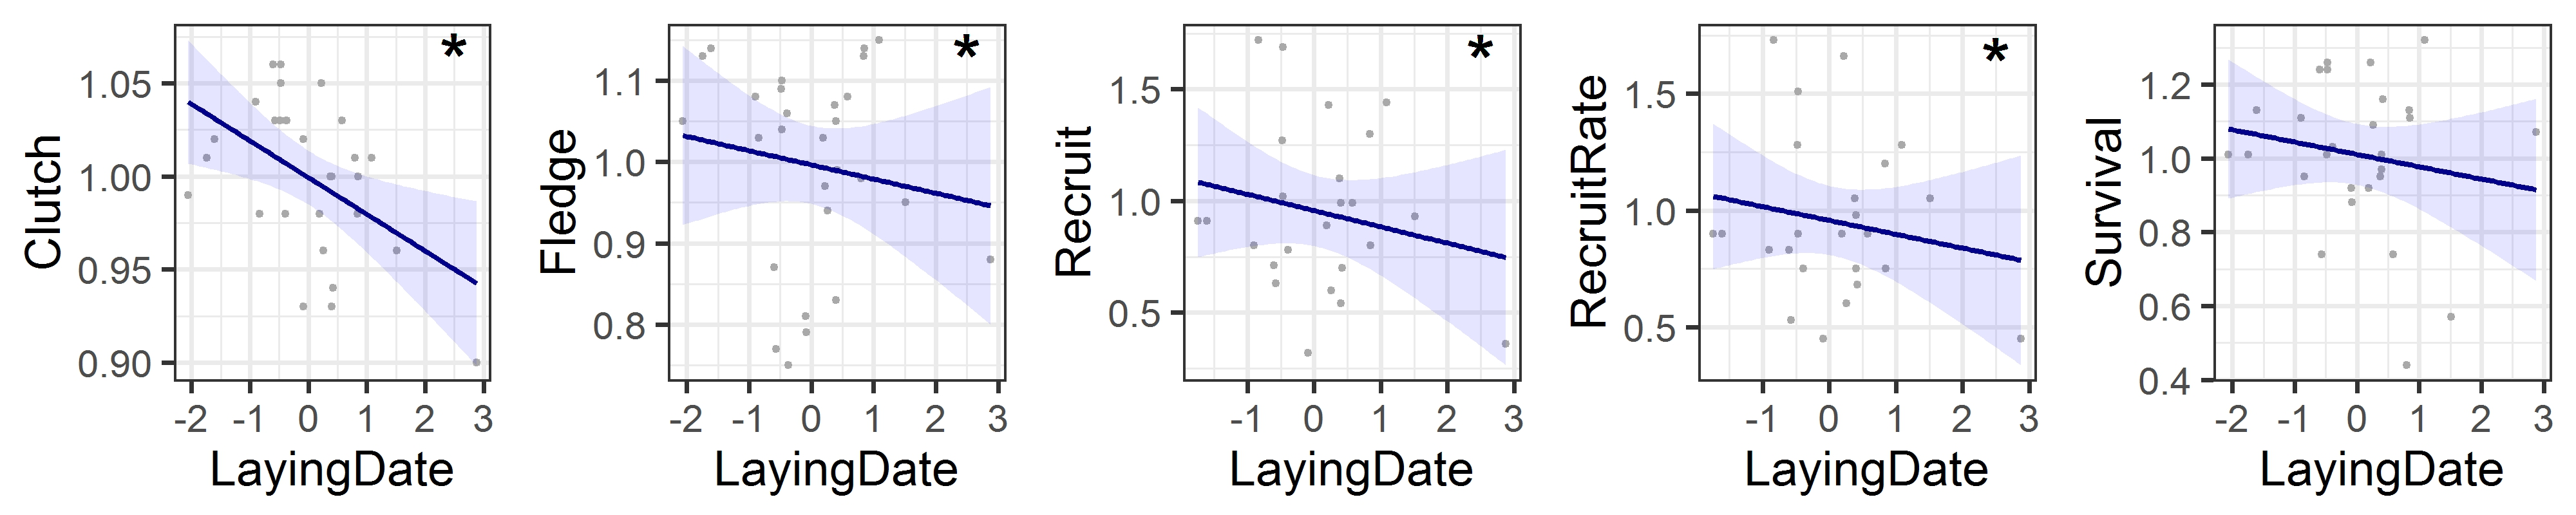
\includegraphics[width=0.90\linewidth]{Figure2_1}
\captionof{figure}{Directional selection coefficients between annual fitness and laying date.}
\end{center}

%------------------------------------------------

None of the annual climatic conditions showed a significant change throughout the study period (p>0.05).
\\
\\
Models on yearly linear selection gradients showed that $\beta$ increases as variation of temperature in April increased, considering clutch size as a proxy of fitness (Figure 3. P<0.01, df=26), while it showed a quadratic relationship with number of feldging (P<0.01, df=25).\\
Regarding the North Atlantic Oscillation in winter, there was a negative association of dry winter on both selection gradients for number of recruits (P=0.02, df=21) and recruitment rate (P=0.02, df=21).

%------------------------------------------------

\begin{center}
%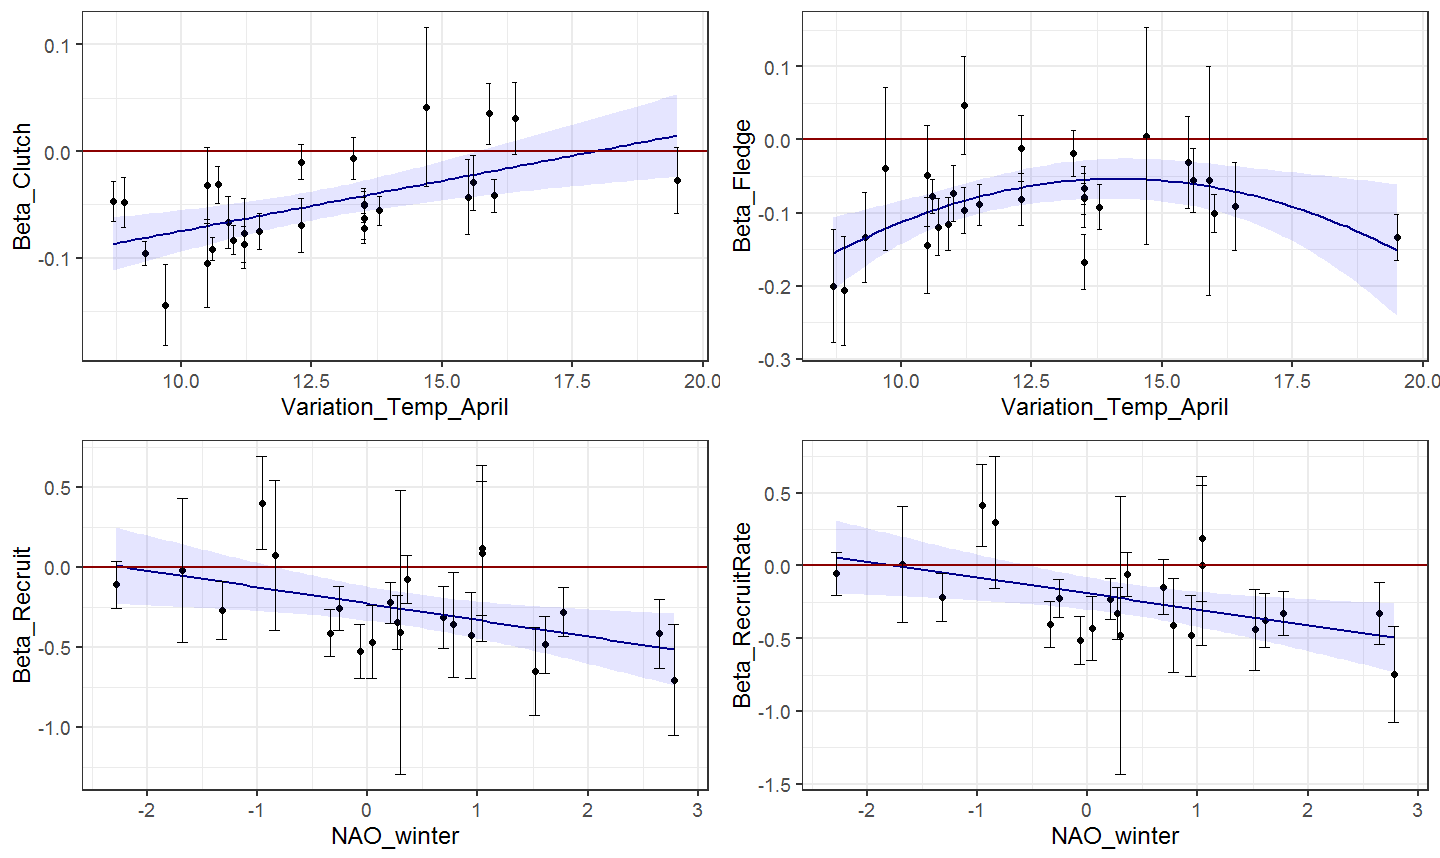
\includegraphics[width=0.90\linewidth]{Figure4}
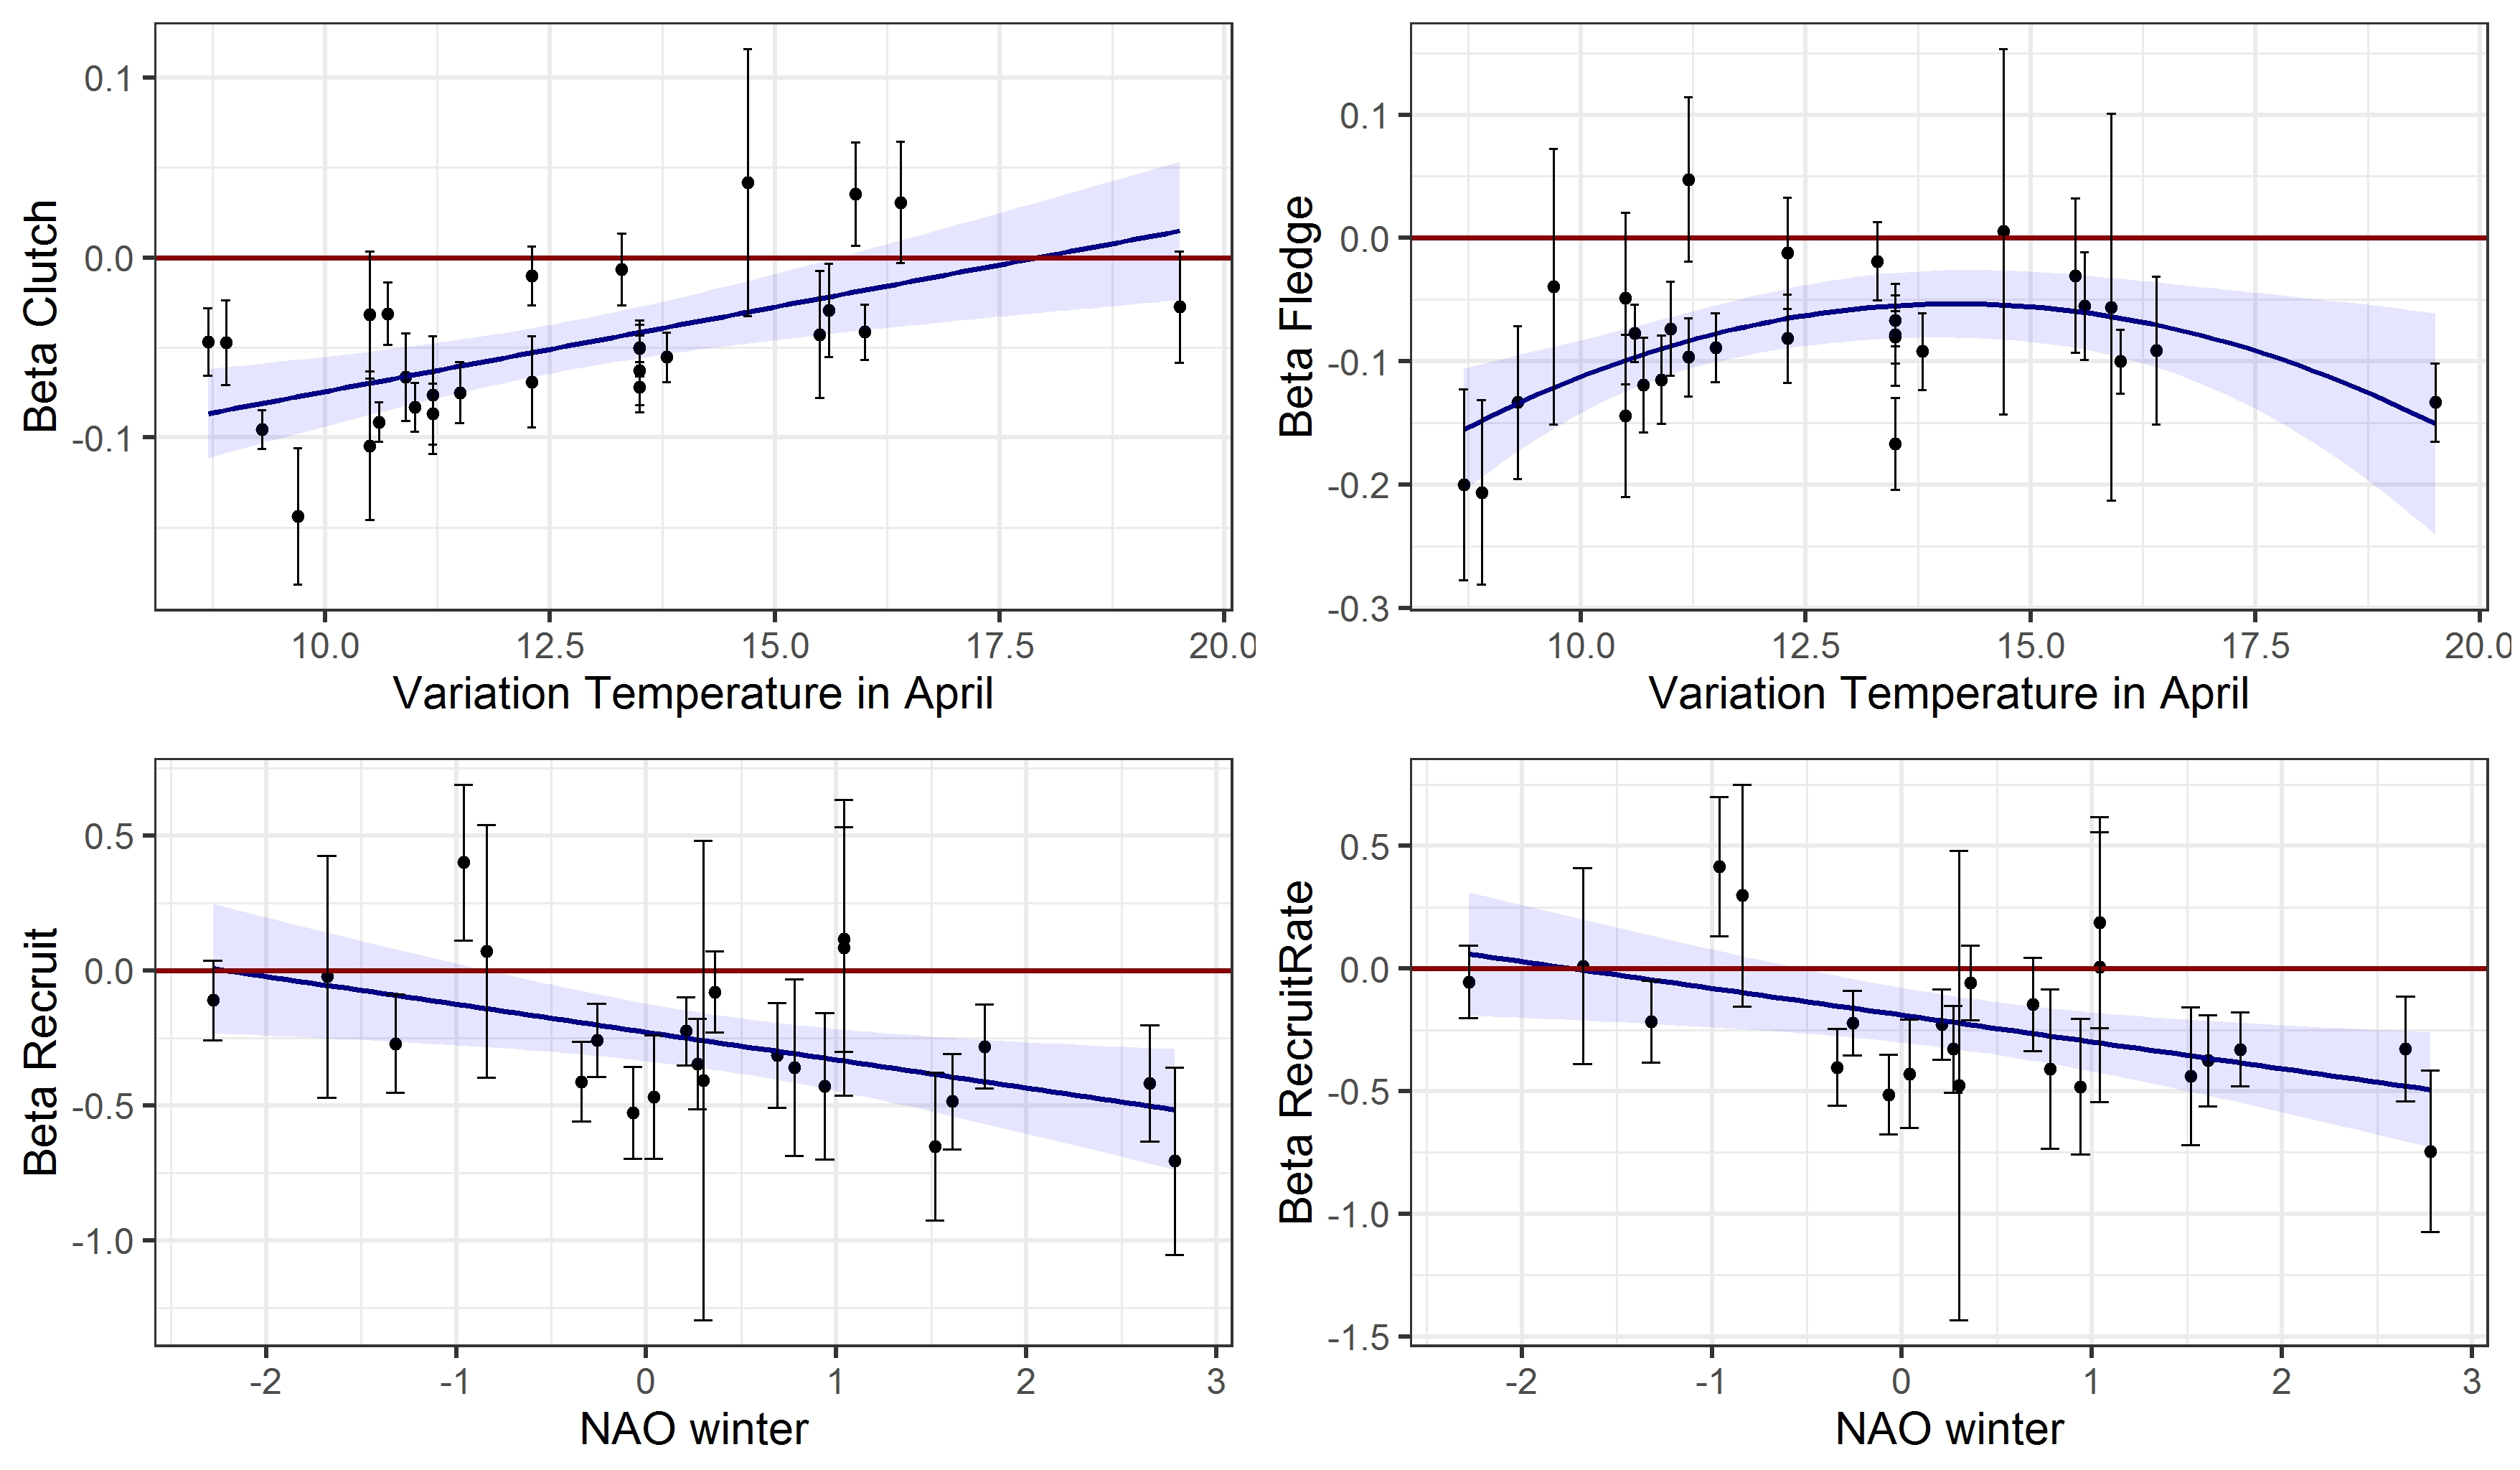
\includegraphics[width=0.90\linewidth]{Figure4_1}
\captionof{figure}{Influence  of agents of selection on linear selection gradients of laying date considering different fitness traits.}
\end{center}
}

%----------------------------------------------------------------------------------------

\end{poster}

\end{document}